\documentclass{beamer}
\usetheme{Boadilla}

\usepackage{amsmath}
\usepackage{amssymb}
\usepackage{amsfonts}
\usepackage{hyperref}
\usepackage{cancel}
\usepackage{multicol}
\usepackage{multirow}

\usepackage{amsmath}
\DeclareMathOperator*{\argmax}{arg\,max}
\DeclareMathOperator*{\argmin}{arg\,min}

\title[Bayesian Inference]{Bayesian Inference under Small Sample Sizes Using General
Noninformative Priors}
\author{Daniil Dorin}
\institute{MIPT, 2024}


\begin{document}
\begin{frame}
    \titlepage
\end{frame}


\begin{frame}
    \tableofcontents
\end{frame}


\section{Motivation}
\begin{frame}{Motivation}
    \begin{block}{Main idea}
    \begin{itemize}
        \item Sample sizes in many engineering fields are often small due to time, economic, and physical constraints. Traditional statistical methods may not be suitable under such conditions.
        \item Bayesian inference is a preferred probabilistic approach in these situations, allowing the integration of prior knowledge with observed data. However, the choice of prior distributions is crucial, especially with limited data, as it can significantly influence the inference results.
        \item This paper introduces a general uninformative prior for Bayesian inference in problems characterized by small sample sizes, aiming to reduce subjectivity and provide objective inference.
    \end{itemize}
    \end{block} 
\end{frame}

\section{Definitions}
\begin{frame}{Definitions}
    Given:
    \begin{itemize}
        \item Likelihood: $p(\mathcal{D}|\mathbf{w})$, $\mathcal{D} = \{\mathbf{X}, \mathbf{y}\}$.
        \item Prior distribution: $p(\mathbf{w}|\mathbf{h})$, probability of the parameters $\mathbf{w}$ given the prior parameters $\mathbf{h}$.
    \end{itemize}
    Posterior distribution $p(\mathbf{w}|\mathcal{D}, \mathbf{h})$:
    $$p(\mathbf{w}|\mathcal{D}, \mathbf{h}) = \frac{p(\mathcal{D}|\mathbf{w})p(\mathbf{w}|\mathbf{h})}{\int p(\mathcal{D}|\mathbf{w})p(\mathbf{w}|\mathbf{h}) d\mathbf{w}}.$$
    Predictive Performance:
    $$p(\mathbf{y}_{\text{test}}|\mathbf{X}_{\text{test}}, \mathbf{y}_{\text{train}}, \mathbf{X}_{\text{train}}) = \int p(\mathbf{y}_{\text{test}}|\mathbf{w}, \mathbf{X}_{\text{test}}) p(\mathbf{w}|\mathbf{X}_{\text{train}}, \mathbf{y}_{\text{train}})d\mathbf{w}$$

\end{frame}
\begin{frame}{Definitions}
    \begin{block}{Uninformative prior}
        If the contribution of the prior is negligible with respect to that provided by the data, then we say that the prior is uninformative. 
        \begin{itemize}
            \item  Jeffreys prior (invariant under reparameterization):
        \[
        p(w) \propto \sqrt{\det I(w)},
        \]
        where \( I(w) \) is the Fisher information matrix. 
        \end{itemize}
    \end{block}
    \begin{block}{Normal-Inverse-Gamma distribution (NIG)}
    Suppose
    \[
    \theta \mid \sigma^2, \mu, \Sigma \sim \mathrm{N}(\mu, \sigma^2 / \Sigma), \quad \sigma^2 \mid \alpha, \beta \sim \Gamma^{-1}(\alpha, \beta).
    \]
    Then \((\theta, \sigma^2)\) has a normal-inverse-gamma distribution, denoted as
    \[
    (\theta, \sigma^2) \sim \text{N-}\Gamma^{-1}(\alpha,\beta,\Sigma,\mu).
    \]
    \end{block}
\end{frame}

\section{Method}
\begin{frame}{Proposed method}
\begin{block}{Assumption}
    Assume the normal likelihood of the data.
\end{block}
\begin{alertblock}{Idea}
        Uninformative priors, including the Jeffreys, Asymptotically Locally Invariant (ALI), for $(\theta, \sigma^2)$ are mostly in the form of $1/\sigma^q$, $q \in {1, 2, \ldots}$ The uniform prior can be seen as a special case of $1/\sigma^q$ as $q = 0$.
\end{alertblock}
    \begin{block}{}
    It is shown as follows that these uninformative priors can be obtained as certain limiting states of NIG conjugates of $(\theta,\sigma^2)$, dim $\theta = k$. For example, the NIG distribution with parameters $(\alpha,\beta,\Sigma,\mu)$ can reduce to the Jeffreys prior:
    \vspace{-0.5cm}
$$
p(\theta,\sigma^2) \rightarrow \frac{1}{\sigma^2}, \quad\text{when}\quad\left\{
\begin{array}{l}
\alpha \rightarrow -k/2 \\
\beta \rightarrow 0^+ \\
\Sigma^{-1} \rightarrow \mathbf{0} \\
|\mu| < \infty
\end{array}
\right.
$$
\end{block}
\end{frame}

\begin{frame}{Proposed method}
Using the conjugacy property of the normal likelihood and the NIG prior, the following estimates are derived:
\vspace{-0.1cm}
       \begin{center}
        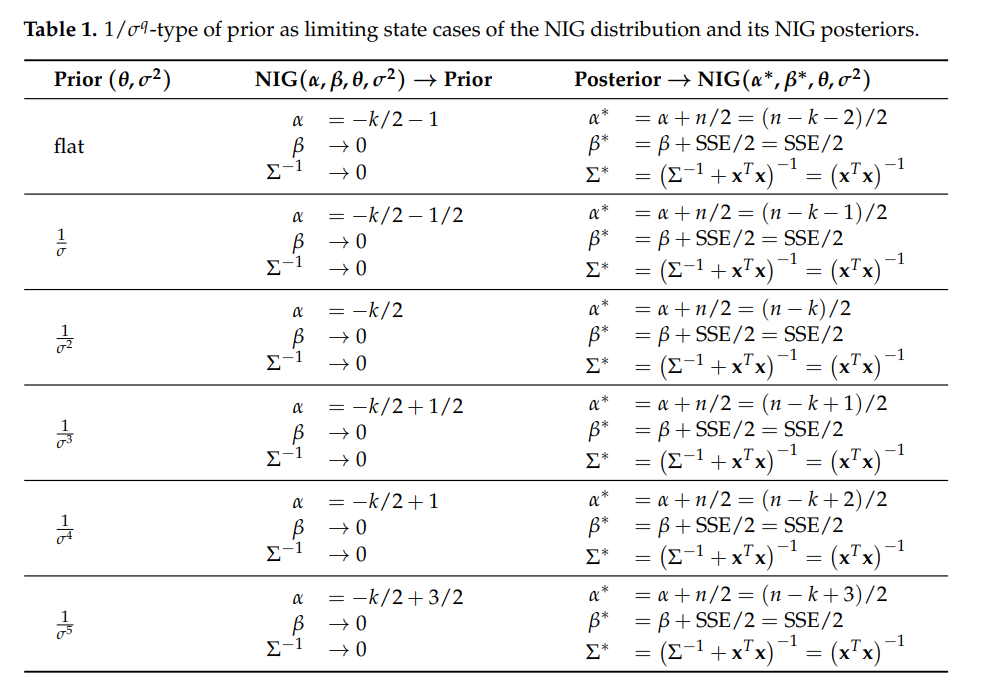
\includegraphics[width=0.83\textwidth]{figs/table.png}
        \end{center}

\end{frame}

\begin{frame}{Proposed method}
\begin{block}{Bayesian prediction}
    In this case, the Bayesian prediction can be calculated analytically:
$$
p(\mathbf{y}_{\text{test}} \mid \mathbf{y}_{\text{train}}) = \mathrm{MVT}_{n-k}\left(
\begin{aligned}
&\mathbf{X}_{\text{test}}(\mathbf{X}_{\text{train}}^T \mathbf{X}_{\text{train}})^{-1}(\mathbf{X}_{\text{train}}^T \mathbf{y}_{\text{train}}), \\
&\frac{\mathrm{SSE}}{n-k}\left(\mathbf{I}+\mathbf{X}_{\text{test}}(\mathbf{X}_{\text{train}}^T \mathbf{X}_{\text{train}})^{-1}\mathbf{X}_{\text{test}}^T\right)
\end{aligned}
\right),
$$
where MVT is multivariate t–distribution. Sum of squared errors is defined as $\mathrm{SSE} = \sum_{i=1}^n (y_i - \mathbf{x}_i^T \boldsymbol{\theta})^2$.
\end{block}
\begin{block}{Advantages of treating the $1/\sigma^q$-type of uninformative prior}
\begin{itemize}
\item The Bayesian posteriors of the model prediction and parameters all have analytical forms, allowing for efficient evaluations without resorting to the MCMC techniques.
\end{itemize}
\end{block}

\end{frame}

\section{Experiments}
\begin{frame}{Experiments}
    \textbf{Data:} The dataset contains data on low-cycle fatigue of materials obtained as a result of tests according to the ASTM E739-10 standard. These data are used to assess the reliability of materials under low-cycle fatigue.
    \vspace{-0.1cm}
       \begin{center}
        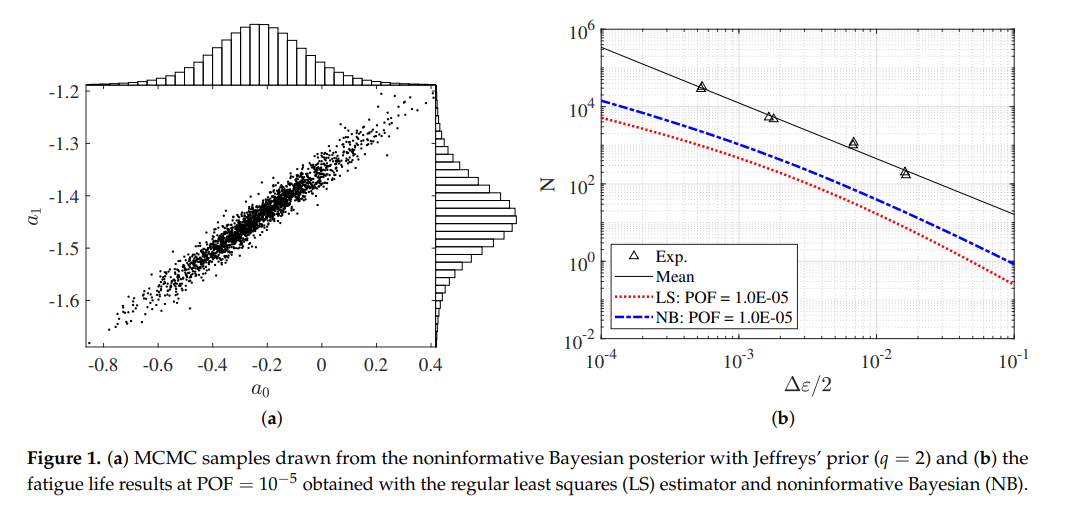
\includegraphics[width=1\textwidth]{figs/exp1.png}
        \end{center}
\end{frame}

\begin{frame}{Experiments}
    \textbf{Data}: Aeroengine Turbine Disk Lifing problem. The number of tested piece is usually less than five due to the cost and time constraints.
    \vspace{-0.1cm}
       \begin{center}
        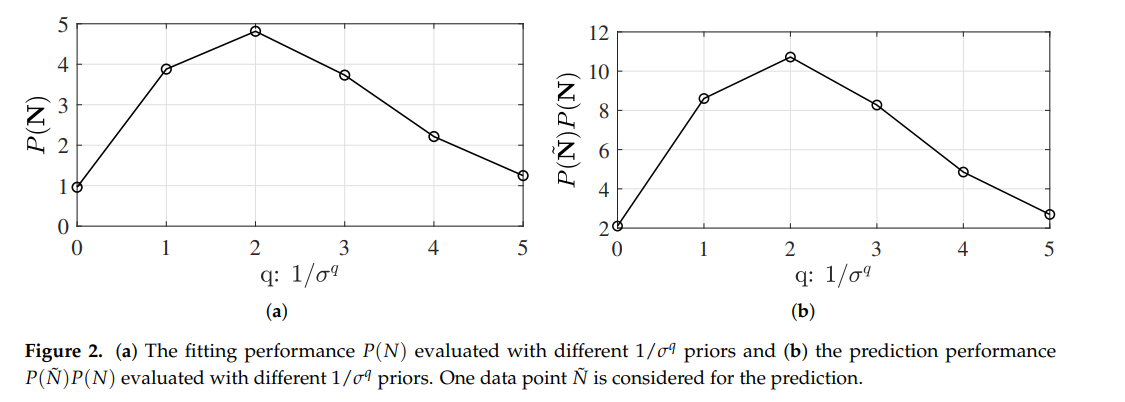
\includegraphics[width=1\textwidth]{figs/exp2.png}
        \end{center}
For the $1/\sigma^q$-type of uninformative prior, the classical Jeffreys prior $1/\sigma^2$ yielded an optimal fitting and prediction performance in terms of the likelihood or Bayes factors.
\end{frame}

\begin{frame}{Experiments}
    Results of uninformative Bayesian (NB) comparable with those obtained
    using the existing method (Ref.) incorporating the empirical evidence and assumptions.
\begin{center}
    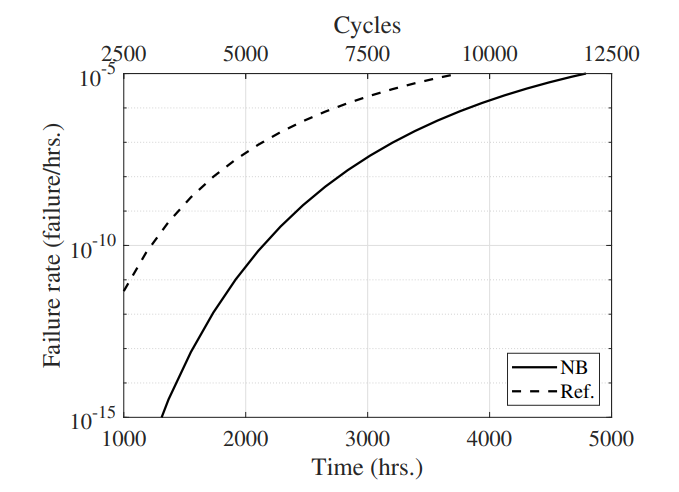
\includegraphics[width=0.6\textwidth]{figs/exp3.png}

\end{center}
\end{frame}

\section{Literature}
\begin{frame}{Literature}
    \begin{enumerate}
        \item \textbf{Main article:} \href{https://www.mdpi.com/2227-7390/9/21/2810}
        {He J. et al. Bayesian inference under small sample sizes using general noninformative priors // Mathematics.}
    \end{enumerate}
\end{frame}

\end{document}